En un proyecto software, las pruebas son una parte fundamental del desarrollo, ya que garantiza que el software funciona
correctamente y se comporta como se espera.\ Además, se asegura que el software no se rompe al añadir nuevas
funcionalidades o al modificar las existentes.\ Existen varios tipos de pruebas, dependiendo del nivel de abstracción
al que se realicen.\ En este proyecto se han implementado pruebas unitarias y de integración.

\subsect{Pruebas unitarias}{pruebas-unitarias}

Las pruebas unitarias son aquellas que se realizan sobre la unidad más pequeña de código, que en el caso de este
proyecto son los métodos.\ Se dividen en dos tipos:

\subsubsect{Pruebas de caja blanca}{pruebas-caja-blanca}

Las pruebas unitarias de caja blanca son un método de diseño de casos de prueba que se basa en la estructura interna
del código a probar.\ Se centra en la cobertura de las rutas de ejecución del código, es decir, se comprueba que se
ejecuta cada línea de código al menos una vez.\ Para ello, se realizan diagramas de control de flujo de los métodos y se
analiza la \boldFont{complejidad ciclomática}, que es una medida de la complejidad de un programa de
ordenador.\ Este tipo de grafo es dirigido, en el que los
nodos representan grupos de instrucciones y las aristas las posibles rutas de ejecución.\ La complejidad ciclomática
se puede calcular mediante 3 ecuaciones diferentes, que son equivalentes:

\begin{center}
	\begin{equation}
		C = R
		\label{eq:complejidad-ciclomatica-1}
	\end{equation}

	\begin{equation}
		C = E - N + 2
		\label{eq:complejidad-ciclomatica-2}
	\end{equation}

	\begin{equation}
		C = D + 1
		\label{eq:complejidad-ciclomatica-3}
	\end{equation}
\end{center}

Donde:
\begin{itemize}
	\item $C$ es la complejidad ciclomática.
	\item $R$ es el número de regiones.
	\item $E$ es el número de aristas.
	\item $N$ es el número de nodos.
	\item $D$ es el número de sentencias de decisión.
\end{itemize}

Cuanto mayor sea la complejidad, más difícil será probar el código y es más probable que contenga errores.
Por ello, se recomienda que la complejidad ciclomática sea menor o igual que 10, para que sea más fácil de
probar~\cite{Cyclomat84:online}.\ A continuación, se muestran las pruebas unitarias de caja blanca
realizadas para un método que tiene sentencias iterativas y condicionales:

\begin{codeBlock}
	\begin{minted}[
		baselinestretch=1.1,
		fontsize=\footnotesize,
		tabsize=2,
	]{java}
				public double probabilityOfClass(NSFWClass nsfwClass) {
					double probability = 0.0;

					for (NSFWClass value : NSFWClass.values()) {
						String predictionName = value.name().toLowerCase();
						probability = this.predictions.get(predictionName).getAsDouble();

						if (value.equals(nsfwClass)) {
							break;
						}
					}

					return probability;
				}
	\end{minted}
	\caption{Método para determinar la clase NSFW asociada a una imagen.}
\end{codeBlock}
\label{cod:codigo-pruebas-unitarias-caja-blanca}

El análisis de la complejidad ciclomática quedaría de la siguiente forma:

\begin{figure}[H]
	\centering
	\begin{tikzpicture}[
		node distance = 1.5cm,
		auto,
		font=\scriptsize,
		every state/.style={circle, draw, minimum size=5mm}
	]
		\node (q1) [state, initial] {$1 \left( hasNext \right)$};
		\node (q2) [state, right = of q1] {$2 \left(for\right)$};
		\node (q3) [state, below right = of q2] {$3$};
		\node (q4) [state, below = of q3] {$4 \left(if\right)$};
		\node (q5) [state, below = of q4, accepting] {$5$};

		\node (r1) [state, right = of q3, draw=none, text=blue] {$\underline{R_1}$};
		\node (r3) [state, left = of q4, draw=none, text=blue] {$\underline{R_3}$};

		\path [-stealth]
		(q1) edge node [text=green!60!black] {$true$} (q2)
		(q1) edge [bend right = 40] node [text=red!60!black, swap] {$false$} (q5)
		(q2) edge node {} (q3)
		(q2) edge [draw=none, bend right=15, text=blue] node {$\underline{R_2}$} (q4)
		(q3) edge node {} (q4)
		(q4) edge node [text=green!60!black] {$true$} (q5)
		(q4) edge [bend left] node [text=red!60!black] {$false$} (q2);

	\end{tikzpicture}
	\caption{Grafo de control de flujo del método \monoFont{probabilityOfClass}.}
	\label{fig:grafo-control-flujo-pruebas-unitarias-caja-blanca}
\end{figure}

Los resultados para cada ecuación son los siguientes:

\begin{itemize}
	\item Ecuación~\ref{eq:complejidad-ciclomatica-1}: $= 3$
	\item Ecuación~\ref{eq:complejidad-ciclomatica-2}: $= 6 - 5 + 2 = 3$
	\item Ecuación~\ref{eq:complejidad-ciclomatica-3}: $= 2 + 1 = 3$
\end{itemize}

Como se puede observar, el método tiene una complejidad ciclomática de 3, por lo que es fácil de probar.\ Ahora se
procede a realizar los casos de prueba para que cada línea de código se ejecute al menos una vez:

\begin{enumerate}
	\item \boldFont{Camino 1}: $1 \rightarrow 5$.
	\\
	\underline{Aristas cubiertas}: $1 \rightarrow 5$.\\
	\underline{Condición}: El enumerado \monoFont{NSFWClass} está vacío.\\
	\underline{Caso de prueba}: \monoFont{nsfwClass} $=$ \monoFont{null}.\\
	\underline{Descripción}:
	Debido a que el enumerado está vacío, no se entra en el bucle y se devuelve el valor por defecto de la variable
	\monoFont{probability}, que es $0.0$.

	\item \boldFont{Camino 2}: $1 \rightarrow 2 \rightarrow 3 \rightarrow 4 \rightarrow 5$.
	\\
	\underline{Aristas cubiertas}: $1 \rightarrow 2$, $2 \rightarrow 3$, $3 \rightarrow 4$, $4 \rightarrow 5$.\\
	\underline{Condición}: \monoFont{nsfwClass.name} $=$ \monoFont{value.name}.\\
	\underline{Caso de prueba}: \monoFont{nsfwClass} $=$ \monoFont{NSFWClass.NEUTRAL}.\\
	\underline{Descripción}:
	El valor del parámetro del método es igual al primer valor del enumerado,
	por lo que se ejecuta la rama \monoFont{true} del condicional y se sale del bucle en la primera iteración.

	\item \boldFont{Camino 3}: $1 \rightarrow 2 \rightarrow 3 \rightarrow 4 \rightarrow 2 \rightarrow 3 \rightarrow 4 \rightarrow 5$.
	\\
	\underline{Nueva arista cubierta}: $4 \rightarrow 2$.\\
	\underline{Condición}: \monoFont{nsfwClass.name} $\neq$ \monoFont{value.name}.\\
	\underline{Caso de prueba}: \monoFont{nsfwClass} $=$ \monoFont{NSFWClass.DRAWINGS}.\\
	\underline{Descripción}:
	El valor del parámetro del método es distinto al primer valor del
	enumerado (en este caso es el segundo), por lo que se ejecuta la rama \monoFont{false} del condicional y se
	vuelve a ejecutar el bucle, saliendo en la segunda iteración.
\end{enumerate}
\label{itm:casos-prueba-pruebas-unitarias-caja-blanca}

\subsubsect{Pruebas de caja negra}{pruebas-caja-negra}

Las pruebas de caja negra son aquellas que se enfocan en la funcionalidad del programa, sin tener en cuenta su
implementación interna.\ Para ello, se diseñan casos de prueba que cubran todas las posibles
\boldFont{entradas y salidas} del programa.
La realización de estas pruebas conlleva la creación de un conjunto de datos de prueba, que se
organizan en \boldFont{clases de equivalencia} (o particiones de equivalencia) y
\boldFont{condiciones límite}.\ En este caso, se han diseñado los casos de
prueba usando la técnica de particiones de equivalencia, que consiste en dividir el conjunto de datos de entrada en
subconjuntos de datos de entrada válidos e inválidos, de tal forma que se garantice que todos los casos de prueba
se validan una vez.\ A continuación, se muestran las clases de equivalencia definidas para la funcionalidad de
consultar los emojis en función de su nombre:

\begin{table}[H]
	\centering
	\caption{Definición de las clases de equivalencia.}
	\begin{adjustbox}{width=\textwidth}
		\begin{tabular}{|c|c|c|c|c|c|c|}
			\hline
			\multirow{2}{*}{\boldFont{Sec.}} & \multirow{2}{*}{\begin{tabular}[c]{@{}c@{}}
																   \boldFont{Condición}\\ \boldFont{de entrada}
			\end{tabular}} & \multirow{2}{*}{\boldFont{Tipo}} & \multicolumn{2}{c|}{\boldFont{Clases válidas}} & \multicolumn{2}{c|}{
				\boldFont{Clases No Válidas}} \\ \cline{4-7}
			& &        & \textit{Entrada} & \textit{Código}           & \textit{Entrada} & \textit{Código} \\ \hline
			& & Lógico & Cadena vacía     & CEV\textless1\textgreater &                  &                 \\ \cline{
				3-7}
			\multirow{2}{*}{1} & \multirow{2}{*}{Nombre de emoji} & \multirow{3}{*}{Si está, es Valor} &
			Cadena con caracteres válidos & CEV\textless2\textgreater & \begin{tabular}[c]{@{}c@{}}
																			Cadena con caracteres válidos pero \\ no
																			existe en base de datos
			\end{tabular} & CENV\textless1\textgreater \\ \cline{4-7}
			& & & & & \begin{tabular}[c]{@{}c@{}}
						  Cadena con caracteres no\\ soportados (números, /, ?, !, etc.)
			\end{tabular} & CENV\textless2\textgreater \\ \hline
		\end{tabular}
	\end{adjustbox}
	\label{tab:clases-equivalencia-caja-negra}
\end{table}

\begin{table}[H]
	\centering
	\caption{Casos de prueba para la funcionalidad de consultar emojis por nombre.}
	\begin{adjustbox}{width=\textwidth}
		\begin{tabular}{|c|c|c|c|}
			\hline
			\multirow{2}{*}{\boldFont{ID CP}} & \multirow{2}{*}{\boldFont{Escenario}} & \boldFont{Condiciones de
			entrada} & \multirow{2}{*}{\boldFont{Resultado esperado}} \\ \cline{3-3}
			& & \textit{Nombre de emoji} & \\ \hline
			CP1 & Escenario 1 & Válida
			& Lista vacía \\ \hline
			CP2 & Escenario 1 & Válida & Lista con emojis cuyo
			nombre contiene la cadena \\ \hline
			CP3 & Escenario 2 & No Válida
			& Lista vacía \\ \hline
			CP4 & Escenario 3 & No Válida & Respuesta HTTP 404 - No
			emojis found \\ \hline
		\end{tabular}
	\end{adjustbox}
	\label{tab:casos-prueba-caja-negra}
\end{table}

\begin{table}[H]
	\centering
	\caption{Valores para los casos de prueba.}
	\begin{adjustbox}{width=\textwidth}
		\begin{tabular}{|c|c|c|c|}
			\hline
			\multirow{2}{*}{\boldFont{ID CP}} & \multirow{2}{*}{\boldFont{Clases de Equivalencia}} & \boldFont{
				Condiciones de entrada} &
			\multirow{2}{*}{\boldFont{Resultado esperado}} \\ \cline{3-3}
			&                           & \textit{Nombre de emoji}              &    \\ \hline
			CP1 & CEV\textless1\textgreater & \textquotedblright \textquotedblright & [] \\ \hline
			CP2 & CEV\textless2\textgreater & \textquotedblright grinning\textquotedblright & [
			\emoji{grinning-cat} ,
			\emoji{grinning-cat-with-smiling-eyes} ,
			\emoji{grinning-face} ,
			\emoji{grinning-face-with-big-eyes} ,
			\emoji{grinning-face-with-smiling-eyes} ,
			\emoji{grinning-face-with-sweat} ,
			\emoji{grinning-squinting-face}
			] \\ \hline
			CP3 & CENV\textless1\textgreater & \textquotedblright emoji\_grin\textquotedblright & 404 - No emojis
			found \\ \hline
			CP4 & CENV\textless2\textgreater & \textquotedblright grin2?\textquotedblright & 404 - No emojis
			found \\ \hline
		\end{tabular}
	\end{adjustbox}
	\label{tab:casos-prueba-caja-negra-con-valores}
\end{table}

\begin{table}[H]
	\centering
	\caption{Nomenclatura utilizada en las tablas de casos de prueba.}
	\begin{tabular}{|c|c|}
		\hline
		\textbf{Código}           & \textbf{Descripción}                 \\ \hline
		CP                          & Caso de prueba                       \\ \hline
		CEV\textless N\textgreater  & Clase de equivalencia válida nº N    \\ \hline
		CENV\textless N\textgreater & Clase de equivalencia no válida nº N \\ \hline
	\end{tabular}
	\label{tab:nomenclatura-casos-prueba-caja-negra}
\end{table}

\subsect{Pruebas unitarias de frontend}{pruebas-unitarias-frontend}

Las pruebas unitarias de frontend se han realizado con Jest, un framework de testing para JavaScript.\ Se han
realizado pruebas para los componentes de React que se utilizan en el perfil de usuario y la alerta de errores.

El componente DropDown debe tener la funcionalidad de estar oculto o visible dependiendo del valor del parámetro
\monoFont{drop}, que se le pasa al componente como propiedad.\ Para ello, se han creado dos pruebas unitarias,
una para cada caso, que comprueban que el componente se renderiza correctamente y que el elemento \monoFont{p} se
muestra o no dependiendo del valor de \monoFont{drop}.

\begin{codeBlock}
	\begin{minted}[
		baselinestretch=1.1,
		fontsize=\footnotesize,
		tabsize=2,
	]{jsx}
						test('Component is not shown with description', () => {
						  const component = render(
						    <DropDown title="Hello" drop={false}>
						      <p>World</p>
						    </DropDown>
						  );

						  expect(component.container).toBeInTheDocument();
						  expect(component.container).toHaveTextContent("Hello");
						  expect(component.container).not.toHaveTextContent("World");
						});
	\end{minted}
	\caption{Prueba unitaria para el componente DropDown cuando \monoFont{drop} es \monoFont{false}.}
	\label{code:prueba-unitaria-dropdown-false}
\end{codeBlock}

\begin{codeBlock}
	\begin{minted}[
		baselinestretch=1.1,
		fontsize=\footnotesize,
		tabsize=2,
	]{jsx}
						test('Component is shown with description', () => {
						  const component = render(
						    <DropDown title="Hello" drop={true}>
						      <p>World</p>
						    </DropDown>
						  );

						  expect(component.container).toBeInTheDocument();
						  expect(component.container).toHaveTextContent("Hello");
						  expect(component.container).toHaveTextContent("World");
						});
	\end{minted}
	\caption{Prueba unitaria para el componente DropDown cuando \monoFont{drop} es \monoFont{true}.}
	\label{code:prueba-unitaria-dropdown-true}
\end{codeBlock}

Cuando se ejecutan todas las pruebas de los componentes con el comando \monoFont{npm run test}, se
obtiene la siguiente salida en consola:

\begin{figure}[H]
	\centering
	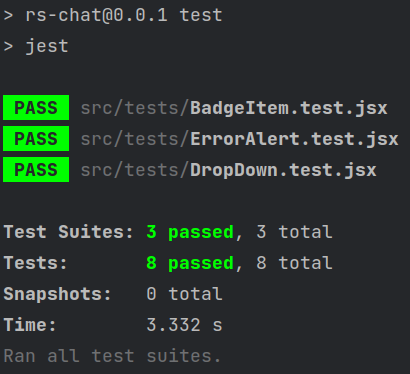
\includegraphics[width=0.4\textwidth]{res/images/pruebas-unitarias-frontend}
	\caption{Salida de las pruebas unitarias de frontend.}
	\label{fig:pruebas-unitarias-frontend}
\end{figure}

\subsect{Pruebas unitarias de backend}{pruebas-unitarias-backend}

Las pruebas unitarias de backend se han realizado con JUnit, un framework de testing para Java.\ Se han
realizado pruebas para cada uno de los diferentes niveles en los que se estructura la aplicación, desde el más
bajo, el de la capa de acceso a datos, hasta el más alto, el de la capa de controladores.\ La técnica utilizada
para la programación de las pruebas ha sido BDD, que consiste en escribir las
sentencias Given-When-Then para cada prueba, de forma que se pueda entender fácilmente qué es lo que se está
probando.

\begin{itemize}
	\item \boldFont{Repositorio}: se han probado todos los repositorios de la aplicación, comprobando que se pueden
	guardar y recuperar los datos de la base de datos.\ Para ello, se ha utilizado una base de datos en memoria
	H2, que se crea y se destruye en cada prueba.\ Estos tests son los más simples, ya que la funcionalidad
	que se prueba es la más básica de la aplicación (acceso a base de datos).\ Las clases de test para los
	repositorios deben tener la anotación \monoFont{@DataJpaTest}, que permite utilizar una base de datos en
	memoria y que se creen los repositorios de forma automática.\ En el código siguiente se puede
	ver un ejemplo de una prueba unitaria para el repositorio de usuarios, en la que se comprueba que se puede
	guardar un usuario en la base de datos y que se puede recuperar por su email.
	\begin{codeBlock}
		\begin{minted}[
			baselinestretch=1.1,
			fontsize=\footnotesize,
			tabsize=2,
		]{java}
	@BeforeEach
	void setUp() {
		this.user = DefaultFactory.INSTANCE.createUser(null, Constants.STUDENT_ROLE);
	}

	@AfterEach
	void tearDown() { this.underTest.deleteAll(); }

	@Test
	void itShouldFindByEmail() {
		// Given
		this.underTest.save(this.user);

		// When
		Optional<User> expected = this.underTest.findByEmail(this.user.getEmail());

		// Then
		assertThat(expected).isPresent();
	}

	@Test
	void itShouldNofFindByEmail() {
		// Given
		// When
		Optional<User> expected = this.underTest.findByEmail(this.email);

		// Then
		assertThat(expected).isEmpty();
	}
		\end{minted}
		\caption{Pruebas unitarias para el método \monoFont{findByEmail} del repositorio de usuarios.}
	\end{codeBlock}

	\item \boldFont{Servicio}: se han probado los servicios de la aplicación, utilizando el framework
	\boldFont{Mockito}, que ofrece la posibilidad de simular el comportamiento de los objetos que tengan la
	anotación \monoFont{@Mock}.\
	\begin{codeBlock}
		\begin{minted}[
			baselinestretch=1.1,
			fontsize=\footnotesize,
			tabsize=2,
		]{java}
@Mock private DegreeRepository degreeRepository;
@Mock private ChatRepository chatRepository;
@Mock private UserChatRepository userChatRepository;
@Mock private SubjectRepository subjectRepository;
@Mock private StudentSubjectRepository studentSubjectRepository;
@Mock private TeacherSubjectRepository teacherSubjectRepository;
private DegreeService underTest;
private Degree degree;

@BeforeEach
void setUp() {
	this.underTest = new DegreeService(
			this.degreeRepository, this.chatRepository,
			this.userChatRepository, this.subjectRepository,
			this.studentSubjectRepository, this.teacherSubjectRepository
	);
	this.degree = new Degree(1L, "Test", emptySet());
}

@Test
void testGetByName() {
	// given
	given(this.degreeRepository.findByName(this.degree.getName()))
			.willReturn(Optional.of(this.degree));

	// when
	this.underTest.getByName(this.degree.getName());

	// then
	verify(this.degreeRepository).findByName(this.degree.getName());
}

@Test
void testSaveDegreeOk() {
	// given
	given(this.degreeRepository.save(this.degree)).willReturn(this.degree);

	// when
	this.underTest.saveDegree(this.degree);

	// then
	ArgumentCaptor<Degree> degreeArgCaptor = ArgumentCaptor.forClass(Degree.class);
	verify(this.degreeRepository).save(degreeArgCaptor.capture());
	Degree capturedDegree = degreeArgCaptor.getValue();
	assertEquals(this.degree.getName(), capturedDegree.getName());
}
		\end{minted}
		\caption{Pruebas unitarias para el servicio de grados utilizando Mockito.}
	\end{codeBlock}
	Las clases de test para los servicios deben tener presente (antes de su definición) la anotación
	\monoFont{@ExtendWith(MockitoExtension.class)}, que permite utilizar las anotaciones de Mockito.\ En el
	código anterior se puede ver un ejemplo de una prueba unitaria para el servicio de grados, en la que se
	comprueba que se puede recuperar un grado por su nombre.\ También se puede observar cómo se simula el
	comportamiento de los repositorios, anotados con \monoFont{@Mock} (para que devuelvan los datos que se quieran)
	y ver los parámetros con los que se llaman a los métodos.
\end{itemize}
\label{itm:pruebas-unitarias-backend}

\subsect{Pruebas de integración}{pruebas-integracion}
% Todo: Pruebas de integración
% Uso mockito...

\subsect{Pruebas de sistema}{pruebas-sistema}
% Todo: Pruebas de sistema, que se han hecho, aunque sea a mano, con Postman
